\documentclass{article}[18pt]
\usepackage{../../../../../format}
\lhead{Coursework}
\usepackage{enumitem}


\begin{document}
\begin{center}
\underline{\huge ADS Coursework}
\end{center}
\setcounter{section}{3}
\section{}
\begin{enumerate}[label=(\alph*)]
	\item Assume that there are constants k and C such that
	$$2x^4\leqslant C\cdot (x^3+3x+2)$$
	when $x\geqslant k$
	$$\dfrac{2}{C}\leqslant \dfrac{1}{x}+\dfrac{3}{x^3}+\dfrac{2}{x^4}$$
	For values of x greater than 1, as the value of x increases $\dfrac{1}{x}+\dfrac{3}{x^3}+\dfrac{2}{x^4}$ tends to 0 and so this does not hold
	\item 
	As $x>\log x$ for all $x>0$
	$$f(x)=4x^3+2x^2\log x+1\leqslant 4x^3+2x^3+1$$
	As $x^3\geqslant 1$ for all $x\geqslant 1$
	$$f(x)=4x^3+2x^2\log x+1\leqslant 4x^3+2x^3+1\leqslant 7x^3$$
	For $x\geqslant 1$. Because the above inequality holds for every positive $x\geqslant 1$, using $k=1$ and $C=16$ as witnesses, we get
	$$|f(x)|\leqslant C\cdot |x^3|$$
	For every $x\geqslant k$
	\item 
	$$f=\omega(g)\Leftrightarrow g=o(f)$$
	So by proving that
	$$x\log x=o(3x^2+7x+1)$$
	It is true that
	$$3x^2+7x+1=\omega (x\cdot \log x)$$
	That would be true if:
	$$\lim_{x\rightarrow \infty}\dfrac{x\log x}{3x^2+7x+1}=0$$
	As $x>\log x \quad \forall \quad x>0$ if $\lim_{x\rightarrow \infty}\dfrac{x^2}{3x^2+7x+1}=0$ then $\lim_{x\rightarrow \infty}\dfrac{x\log x}{3x^2+7x+1}=0$\\
	As $x^2<3x^2+7x+1$ then $x>\log x \quad \forall \quad x>0$ if $\lim_{x\rightarrow \infty}\dfrac{x^2}{3x^2+7x+1}=0$
	Therefore 
	$$3x^2+7x+1=\omega (x\cdot \log x)$$
	With the witness $k=1$ and $C=1$
	\item 
	$f(x)=x^2+4x$\\
	$g(x)=x\cdot \log x$
	$$|f(x)|\geqslant C\cdot |g(x)|$$
	As for $x>0 \ x>\log x$
	$$x^2+4x\geqslant x^2 \geqslant x\cdot \log x$$
	So it is true with the witnesses $c=1$ and $k=1$
	\item 
	As you don't know anything about the complexity of $f(x)$ and $g(x)$ it is impossible to say what the complexity of their sum is
\end{enumerate}
\section{}
\begin{enumerate}[label=(\alph*)]
	\item 
	$$T(n)=9T\bigg(\dfrac{n}{3}\bigg)+n^2$$
	$a=9, b=3, f(n)=n^2, \log_ba=2$
	$$f(n)=\Theta(n^2)$$
	$$T(n)=\Theta(n^2\log n)$$
	\item 
	$$T(n)=4T\bigg(\dfrac{n}{2}\bigg)+100n$$
	$a=4,b=2,f(n)=100n, \log_ba=2$
	$$f(n)=\mathcal{O}(n^{2-1})$$
	$$T(n)=\Theta(n^2)$$
	\item As a is not a number this cannot be solved using master theorem
	\item 
	Under the assumption that c is a constant, otherwise this cannot be solved using master theorem
	$$T(n)=3T\bigg(\dfrac{n}{3}\bigg)+c\cdot n$$
	$a=3,b=3,f(n)=c\cdot n,\log_ba=1$	
	$$f(n)=\Theta(n^1)$$
	$$T(n)=\Theta(n\log n)$$
	\item 
	$$T(n)=0.99T\bigg(\dfrac{n}{7}\bigg)+\dfrac{1}{n^2}$$
	$a<1$ so Master theorem cannot be performed
\end{enumerate}
\newpage
\section{}
(b)\\
Suppose you want an output to be the list of length 8
$$[7,6,5,4,3,2,1,0]$$
For this to be the worst case for the merge, the two lists of length four to be merged should run out at the same time. So the lists should be List A: $[7,5,3,1]$ and List B: $[6,4,2,0]$.\\
\\
Selection sort has no worst case, as the same number of comparisons will be used for any list of a given length. So just for example, the input to selection sort is the numbers in ascending order, but those numbers could be in any order for a worst case of the algorithm.
\\
For these two sublists to be produced from a list of length 8, each half should be one of the sublists, so a worst case for a list of length 8 would be.
$$[1,3,5,6,0,2,4,6]$$
Below is a demonstration of the algorithm running on that input list
\begin{center}

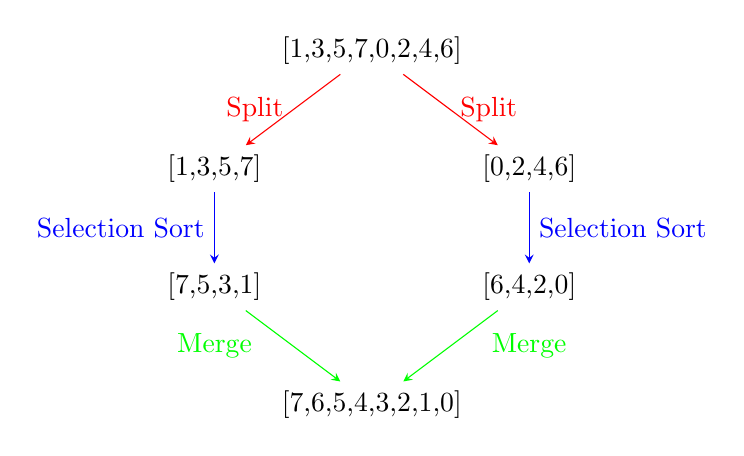
\begin{tikzpicture}[node distance=2cm]
\tikzstyle{arrow} = [->,>=stealth]

% nodes
\node (A) at (0, 0.5) {[1,3,5,7,0,2,4,6]};
\node (B) at (-2, -1) {[1,3,5,7]};
\node (C) at (2, -1) {[0,2,4,6]};
\node (D) at (-2, -2.5) {[7,5,3,1]};
\node (E) at (2, -2.5) {[6,4,2,0]};
\node (F) at (0, -4) {[7,6,5,4,3,2,1,0]};
% arrows

\draw [arrow,red] (A) -- node[anchor=east] {Split} (B);
\draw [arrow,red] (A) -- node[anchor=west] {Split} (C);
\draw [arrow,blue] (B) -- node[anchor=east] {Selection Sort} (D);
\draw [arrow,blue] (C) -- node[anchor=west] {Selection Sort} (E);
\draw [arrow,green] (D) -- node[anchor=east,xshift=-4mm] {Merge} (F);
\draw [arrow,green] (E) -- node[anchor=west,xshift=4mm] {Merge} (F);


\end{tikzpicture}

\end{center}

\end{document}